\documentclass[uplatex,twocolumn]{jsarticle}
\setlength{\columnsep}{8mm}
\usepackage[dvipdfmx]{graphicx}
\title{タイトル}
\author{著者}
\date{\parbox{.8\textwidth}{
  \noindent\hfil{\bfseries\abstractname}\hfil\\\indent
  ここに概要を書く。この文書は研究室内シンポジウムのための雛形文書です。と
  か。
}}
\pagestyle{empty}

\begin{document}
%\setcounter{page}{15} %開始ページを設定
\maketitle
\thispagestyle{empty}

\section{セクション}

\subsection{サブセクション}
参考文献の参照\cite{bunken1}
\subsubsection{サブサブセクション}
\section{脚注}
脚注はページの下の方にでます\footnote{こんなふうに}。


\section{図}
図\ref{aco}を示す。\\

\begin{figure}[htbp]
 \begin{center}
  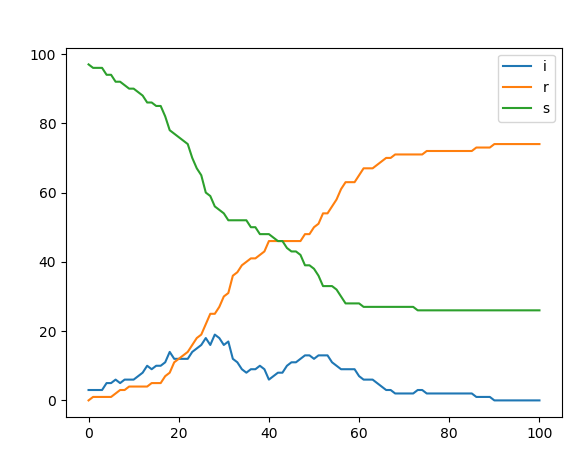
\includegraphics[width=6cm]{fig1.png}
 \end{center}
 \caption{謎のグラフ}
 \label{aco}
\end{figure}

\section{表}

表\ref{tenki}を示す。

\begin{table}[htbp]
\begin{center}
 \caption{天気}
 \label{tenki}
 \begin{tabular}{|l|p{5zw}|p{5zw}|}\hline
  日付 & 午前           & 午後               \\ \hline
  9/1  & はれ           & はれときどきくもり \\ 
  9/2  & くもりのちあめ & あめ               \\ 
  9/3  & はれ           & はれ               \\ \hline
 \end{tabular}
 \end{center}
\end{table}


\begin{thebibliography}{99}
 \bibitem{bunken1} 著者, 参考文献タイトル.
\end{thebibliography}
\end{document}
